\index{Database!Log-in}
\index{Log-in!Database}
\begin{enumerate}
\item \gdprojects{} are stored in  a \gddb{}. Before you can access a \gdproject{}, you have to log in to the \gddb{}. 
\item The log-in dialog for the \gddb{} (\bxfigref{dblogin}) appears automatically the first time you need it (e.g. when you try to open or create a \gdproject{}). 

\begin{figure}[h]
\begin{center}
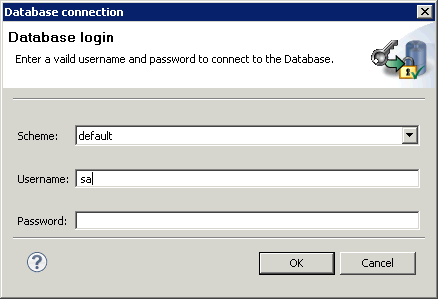
\includegraphics[width=10cm]{Tasks/Database/PS/dblogin}
\caption{Database login}
\label{dblogin}
\end{center}
\end{figure}

\bxtipp{If you are using the default demo (embedded) \gddb{}, you will automatically be logged into the \gddb{}. }

\item Select the \gddb{} you want to use and enter your username and password.

\bxtipp{If you previously had another \app{} version installed, you may see the information that your current \gddb{} version is not compatible with the latest version. If this is the case, then you can automatically migrate your \gddb{} \bxpref{DBMigrate}.}
\end{enumerate}

